\section{The Communication of Information and Knowledge: An
Important Facet of Lifelong Learning} \shorttitle{Communication of Information and Knowledge}

Media are (external) information storage devices and transmitters. Knowledge is the internal representation of information including the relations of all the components in a living being. Lifelong learning means acquiring knowledge at all stages of life. Three different kinds of knowledge - among others - can be identified: 
\begin{itemize}
	\item Procedural knowledge (e.g., setting the VCR-timer).
	\item Social and semantic knowledge (e.g., Alois Alzheimer was born in 1864). 
	\item Personal knowledge (e.g., what wartime was like).
\end{itemize}

The human species is the only species that can transfer knowledge by an elaborate system of communication. Humans learn throughout all their life, they are able to plan ahead by imagining, rehearsing and evaluating situations. Humans can do that mentally, in games and by watching or listening to others - even by reading a book, surfing the internet, listening to radio or watching TV or a movie. 

 Our overarching research question is what roles media play for lifelong learning and if age differences can be identified.

\subsection{BALANCE: The Effects of Media Communication}

\index{Schwender, Clemens}

\paragraph{Research Team}
Clemens Schwender (Professor), Siegmar Otto (Doctoral Fellow), Dennis Mocigemba (Postdoctoral Fellow), Aynur Huylu (Dipl. Media Consultant), Claudia Hesping (Dipl. Media Consultant), Hatice Ecirli (Student Assistant), Florin Bora (Student Assistant)

 Project BALANCE: Why do people turn off the TV? This is the question that the BALANCE project tries to answer with regard to sustainability communication on TV. Sustainability communication faces the criticism that it reaches only those, who are informed anyway, and that a great part of society is not reached at all. Viewers turn off, or switch between channels and thereby refuse reception. The BALANCE project tries to change that by developing and implementing the concept of ecotainment: Messages about sustainability are to be combined with positive emotions.

 By applying content analysis (to identify narrative structure, offered messages and symbols for ecology and sustainability) as well as on- and offline questionnaires (to identify emotional impact, memory and attitudes toward the presented messages), we develop concepts for educational materials and inform journalists and production teams about our findings. The ultimate goal of the project is to broaden knowledge about sustainability in the population.

\null
\textbf{Research Highlights 2006}

\textit{The Avoidance of Information}

 When people watch TV, they use the remote control to decide about the information they will accept. So far, research on strategies of switching channels was centered mainly on the context of commercial avoidance. In my working group, we have developed a model that is able to determine reasons for switching channels that captures not only the content level, but also other factors, such as film aesthetics. The goal is to develop different categories to improve knowledge transfer, especially within the informal context of mass communication.

 Since Fall 2006 we finally have access to media ratings on a second-by-second basis. Now we will be able to find the moments (and reasons) when (and why) people switch channels while watching reports that contain knowledge information. The reasons can be clustered in three domains: (a) Context (like position of the episode, the position in relation to commercial breaks, the program of competitive channels), (b) Content (like interview situations, the presentation of big machines and production lines, the three dimensions - social, ecological and economical - of sustainability), and (c) Formal Aspects (like duration, number of cuts per minute). Our preliminary results indicate that an episode is accepted when it fits the viewers expectations in respect to the program. In the context of ``Welt der Wunder'' sustainability is an accepted topic. 

\textit{Investigation of Media Strategies for Audio-Visual Arguments}

 My working group is also investigating a representative sample of TV-Commercials to better understand what strategies media use for making audio-visual arguments. The term ``narrative function'' is able to explain how characters are used. For the first time, the categories age and gender are not used in content analysis to determine the respective demographic representation, but to determine their function as a stereotypical argument. The goal is to learn how commercials succeed in making a convincing audio-visual argument in a very short time.

 The content analysis of 698 TV-spots for products and services but also for social behavior or awareness and for political parties is finished. The spots present more than 5.000 agents.

\textit{Investigation of the Public Debate on Sustainability in TV and Print Media}

 With the support of ``google news'' we are able to check 700 papers daily for the terms ``sustainability'' and ``sustainable development''. Long-term studies were made with the daily paper ``Die Tageszeitung'' and the weeky paper ``Die Zeit'' from 2002 to 2005. The data show that great events like the Johannesburg World summit in 2002 had a verifiable impact on the coverage of sustainable development in Germany.

 Twice a year, we look at a TV Guide to detect all possible shows that may include issues that deal with sustainability. The media survey suggests a bigger potential for public debate on sustainability.

\newpage
\textit{Transfer of results}

 We are currently preparing a series of workshops for journalists as well as for experts in the field of sustainability research. The workshops will be organized by the Adolf-Grimme-Institut (Marl) and the Bundespressekonferenz (Berlin). 


\paragraph{Collaborations}
\begin{itemize}
\item Universit\"at Hohenheim \\ Lehrstuhl Umweltmanagement \\ Prof. Dr. Werner F. Schulz; Martin Kreeb; Volker Diffenhard 
\item Copenhagen Business School \\ nwd Institut \\ Dr. Lucia Reisch 
\item .lichtl Sustainability Communications \\ Martin Lichtl
\item Adolf-Grimme-Institut, Marl \\ Dr. Friedrich Hagedorn 
\end{itemize}

\begin{bibunit}[apalike]
\nocite{*}
\putbib[profClemensSchwender]
\end{bibunit}

\paragraph{Grants}

\begin{itemize}
\item BMBF (PI: C. Schwender). B.A.L.A.N.C.E. Development, Application and Promotion of a Communicational and Trendsetting Concept for a Sustainable Life and Management 2004-2006.
\end{itemize}

\newpage
\subsection{Technical Documentation: Age-related Formatting of Information}

\index{Schwender, Clemens}

\paragraph{Research Team}
Clemens Schwender (Professor), Christoph K\"{o}hler (Dipl. Media Consultant), Ulrich B\"{u}hring (Student Assistant Donau University Krems).

 In our homes and at work we are confronted with new technology. Written, AV- or online-documentations explain how to build or handle these artefacts. Again and again we are faced with situations in which technology is not self-explaining but needs introduction instead. Media-based teaching happens without the presence of a teacher. People must read and understand text and pictures. Formatting and design play crucial roles in the motivation to access user's manuals. There is no option of asking questions and receiving immediate answers. Manuals must reflect the restrictions and preferences of the users of different age, gender and cultural background.

\begin{figure}[h]
  \begin{center}
    \begin{minipage}[b]{0.35\linewidth}
   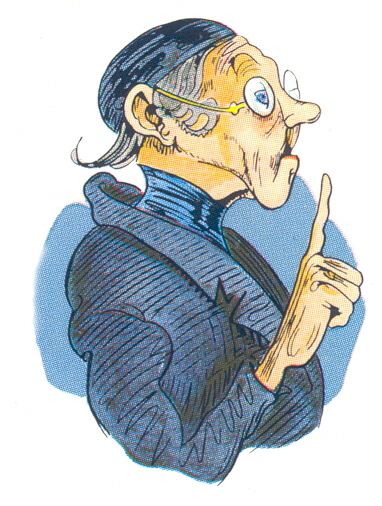
\includegraphics[width=\linewidth]{profClemensSchwender-fig1.jpg}
    \end{minipage}\hfill
    \begin{minipage}[b]{0.55\linewidth}
      \caption{Taken from Wilhelm Busch (1865): Max und Moritz. This kind of humorous dispersal is not accepted in technical documentation.\label{fig1:profClemensSchwender}}
    \end{minipage}
  \end{center}
\end{figure}

 Technical documentation is usually associated with boring reading. People avoid taking the manuals in their hands. We are investigating how motivation can be improved by making changes in the design: The page layout, font type and font size are considered as well as the use of more pictures and pictures that portrait not only machines but also people. The role of humor will be tested, to see if it has an influence on the motivation to look at a manual and to read it.

\null
\textbf{Research Highlights 2006}

 The research on technical documentation is a prototype for learning in adulthood. Technical documentation is an important example of lifelong learning. We try to observe how the learning process takes place without the presence of a teacher. In our working group we look at the formatting of information and test different conditions with persons of different age. 

 First results indicate that color and font size play a positive role and can be considered as motivational factors. Humor and comic-style pictures provoke resistance against the documentation. Effects on the speed of transforming reading into action and the accuracy of accomplishment cannot be found.


\paragraph{Collaborations}
\begin{itemize}
\item tekom - Der deutsche Fachverband f\"{u}r Technische Kommunikation und Informationsentwicklung
\end{itemize}

\begin{bibunit}[apalike]
\nocite{*}
\putbib[profClemensSchwender2]
\end{bibunit}

\subsection{Feldpost-Archiv} 

\index{Schwender, Clemens}

\paragraph{Research Team}
Clemens Schwender (Professor), Thomas Jander (Student Assistant, Humbold University Berlin), Dr. Jens Ebert (Literature Historian), Elena Nedbaylo (PhD Candidate), Dr. Ortwin Buchbender (Military Historian)

 The Feldpost-Archiv is an archive for the war time generation's personal knowledge. Media are used to communicate experience, opinions, and knowledge. E-mails, letters, and the telephone are examples of individual media. The problem of investigating their content and usage is that they are usually not stored, but forgotten, deleted or thrown away - with one unique exception: Feldpost letters. With the Feldpost Collection, Feldpost letters will be catalogued and coded for scientific use. The data will be accessible over the Internet. The goal is to build a representative, web-based collection of war letters.

 Personal memories, experiences and written statements of the war generation are a valuable subject for research on memory and media, as well as for political psychology. Based on such collections, for instance, background questions about the age-graded effects of propaganda can be asked and hopefully answered in the near future. 

\begin{figure}[h]
  \begin{center}
    \begin{minipage}[b]{0.40\linewidth}
   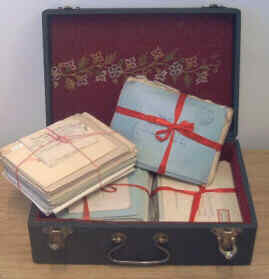
\includegraphics[width=\linewidth]{profClemensSchwender-fig2.jpg}
    \end{minipage}\hfill
    \begin{minipage}[b]{0.55\linewidth}
      \caption{Collection of letters in the Feldpost-Archiv in Berlin, initiated by Clemens Schwender.\label{fig2:profClemensSchwender}}
    \end{minipage}
  \end{center}
\end{figure}

\textbf{Research Highlights 2006}

 This year our work concentrated on a survey of so called ``gray literature''. These are publications and editions of war letters and memoirs by war participants or their relatives. Usually these are not critical editions and lack information on provenance. But nevertheless they are important for war letter research and provide a useful source of information if handled with care.

%\begin{figure}[ht]
%  \begin{center}
%    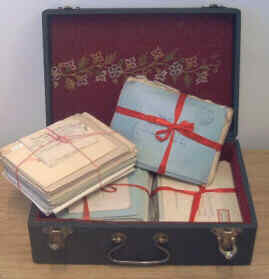
\includegraphics[width=7.5cm]{profClemensSchwender-fig2.jpg}
%    \caption{Collection of letters in the Feldpost-Archiv in Berlin, initiated by Clemens Schwender.}\label{fig2:profClemensSchwender}
%   \end{center}
%\end{figure}

\paragraph{Collaborations}
\begin{itemize}
\item Museum of Communication Berlin \\ Prof. Dr. Joachim Kallinich
\item State Library Stuttgart \\ Prof. Dr. Gerhard Hirschfeld
\item Prussian Cultural Heritage in Berlin, State Library \\ Dr. Jutta Weber 
\item University of Witten/Herdecke \\ Prof. Dr. Harald Welzer
\item State University Surgut, Russia \\ Dr. Vasiliy Glushak
\end{itemize}

\begin{bibunit}[apalike]
\nocite{*}
\putbib[profClemensSchwender3]
\end{bibunit}

\subsection{\mbox{Age, Emotions and Media-Preferences}}

\index{Schwender, Clemens}

\paragraph{Research Team}
Clemens Schwender (Professor).

 People choose what papers they buy, what they read, to what TV-channels they switch, what movies they like and which ones they want to see. This changes during the course of life, but so far no detailed research has been done on this topic.

 Basic answers are still needed: 
\begin{itemize}
	\item Why do people cry, get scared or laugh during movies or while reading a novel?
	\item How and why do preferences change?
	\item Can that be explained by age factors?
\end{itemize}

\null
\textbf{Research Highlights 2006}

 A survey about the reasons why older adults don't go to the movie theaters anymore contained the question about the personal favorite movie. The answers to this particular question raised our interest and led to a broader research question about age-related media- and genre-preferences. The most mentioned movie in the age groups of persons older than 49 is ``Gone with the Wind''.  A wider survey is being conducted. Besides the preferences and the reasons for their selection, there are also items to identify the reception modalities as developed by Monika Suckf\"{u}ll.

%\begin{figure}[ht]
%  \begin{center}
%    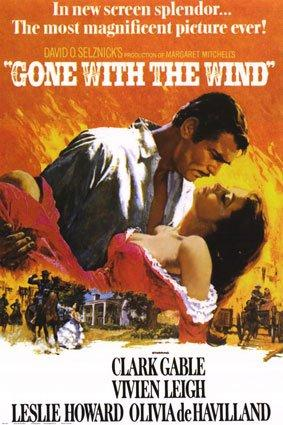
\includegraphics[width=7.5cm]{profClemensSchwender-fig3.jpg}
%    \caption{Most Germans (50+) claim "Gone with the Wind" to be the best movie of all times.}\label{fig3:profClemensSchwender}
%   \end{center}
%\end{figure} 

\begin{figure}
  \begin{center}
    \begin{minipage}[b]{0.40\linewidth}
   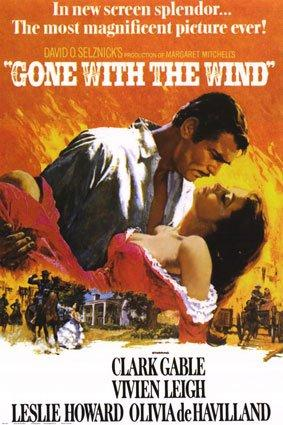
\includegraphics[width=\linewidth]{profClemensSchwender-fig3.jpg}
    \end{minipage}\hfill
    \begin{minipage}[b]{0.55\linewidth}
      \caption{Most Germans (50+) claim "Gone with the Wind" to be the best movie of all times.\label{fig3:profClemensSchwender}}
    \end{minipage}
  \end{center}
\end{figure}


 Preliminary results show that genre preferences change during the lifespan. Preferences change according to age/cohort. Older people favor less aggressive genres like Western, Sciences Fiction or adventure movies. Older people also prefer movies that deal with time periods that they know from their own past experience: Movies about the time and events of World War II are often preferred to movies about contemporary issues. In this category you can find movies like ``The Downfall'' or ``The Boat''. Persons over 70 never mention movies about the future (Science Fiction) as their favorites.

\paragraph{Collaborations}
\begin{itemize}
\item Hochschule f\"{u}r Film \& Fernsehen, Potsdam \\ Dr. Dagmar Hoffmann
\item Universit\"{a}t der K\"{u}nste, Berlin \\ Prof. Dr. Monika Suckf\"{u}ll 
\end{itemize}

\begin{bibunit}[apalike]
\nocite{*}
\putbib[profClemensSchwender4]
\end{bibunit}


\subsection{Identification of Matches and Mismatches in Communication at the Work Place}

\index{Schwender, Clemens}

\paragraph{Research Team}
Clemens Schwender (Professor), Sven Voelpel (Professor)

 Communication is a central part of a company's wealth. Also communication can be a cause for getting sick. We need to identify the factors that support healthy communication styles and how individuals, leadership, and the overall climate can support healthy communication. The balance between asking for and providing information must be identified.
 
\paragraph{Grants}
\begin{itemize}
\item BMBF (PI: JCLL). C. Schwender, S. Voelpel: subproject ``Communication and Experience Management'' within the joint research project ``Effects of Matches/Mismatches between Aspects of Human and Social Capital, Corporate Strategy and Work Organization on the Physical and Mental Well-Being of Employees''.  
\end{itemize}

\enlargethispage{2cm}
\subsection{Other Professional Activities}

\begin{itemize}
\item Reviewer for ICA-Conference in San Fransisco 2007.
\item Reviewer for DGPuK-Conference in Bamberg 2007.	
\end{itemize}
